\chapter{Multicolor registration}
In microscopy it is often desirable to label different structures in a cell with
different colors. To do so our collaborators use different fluoroscent molecules
that emit light at different and distinguishable wavelengths. Using different
filters it is possible to capture pictures just containing light emited from one
fluorophore. To get a mulit-channel picture the different channels must be
aligned. Because different flourophores emit different wavelengths, cromatic
aberration apears. This means that the light for the same spot but with
different wavelenghts is not mapped to the same spot in the image. To align the
different channels despite cromatic aberration, beads are used. Beads are
flourophores added to the probe, that emit light in all wavelengths the
different markers do and therefore are visible in all channels. The beads can be
used as landmarks, because their position in the original image is at the same
spot. The task is to find a transformation that maps corresponding beads on each
other.
\section{Features of the colorcomposer application}
\subsection{Manual bead selection and removal}
With the improved version of the colorcomposer it is possible to add beads manually. Therefore the desired location is clicked in the preview image and after that either the button "add green bead" or "add red bead" is hit. If there are enough frames containing localisations near the given location a bead is added to the center of mass of the intensities in that area. If the button "delete bead" is pressed all beads in the selected area are deleted.\newline
This feature can be used to add beads which the automatic bead detection missed.
\subsection{Automatic bead detection}
The input for the colorcomposer application is a text file created by the storm
algorithm that contains information about the position, intensity, symmetry,
framenumber and signal-to-noise ratio of each detection. The beads should
ideally appear in most of the images, this means they can be found by searching for
detections that appear in almost every frame at the same position.\newline
There was already an automatic bead detection implemented by Joachim Schleicher. This was improved in the following ways.\newline
All important parameters for the bead detection can now be set in the GUI. The bead detection works by searching for points that appear in most of the frames. Instead of taking all localisations from the first frame as expected bead positions without considering locations that does not appear in the first frame, now a good subset of positions from the first 50 frames by skipping redundant positions based on the minimal distance of a new position to all positions already in the set. The range of 50 frames to look for beads is sufficiant because it is very unlikely that all 50 detections of the bead have been missed.\newline
After good candidates are found their number of points, variance and mean position is determined like described by \cite{MAJoachim}.\newline
In the end beads that are too close together are merged to for a new bead with its center right between the merged beads.

\subsection{Alignment of two multicolor images}
\subsection{Information about localisation certainty}
\subsection{Heatmap}


\section{Align Beads}
After the beads for each channel are found the next task is to find the corresponding
beads in each channel. It can happen that some beads occure in just one channel,
if this is the case there will be no corresponding bead in the other
channels.\\
To align the beads, the minimal number of beads, three, that are neccesary to
calculate the transformation are chosen randomly from the first channel. After that, based on
a probabilistic approach and a distance matrix containing information about the
distances between all beads of the two channels, three beads from the
second channel are chosen. It is more likely for nearer beads of the other channel to be selected, but any bead within a certain range can be chosen.\\
Using this pairs of beads a linear transformation is found like described by
\cite{MAJoachim}.\newline
This transformation is used to tested how many other beads, that were not used to calculate the transformation match in
total. It is assumed that the correct transformation will match other bead pairs in addition.
This is very important because with every set of three points a valid transformation can be found that perfectly aligns this three beads. After that the whole
procedure is done multiple times. In the end the best transformation is
chosen based on the total number of bead pairs that match. If there are multiple transformations that match the same number of bead pairs, it is searched for the transformation with the lowest root mean square error for the matching beads.\\
In principle shearing should also be allowed for a linear transformation, but tests
indicate that shearing does not occure, so it is disabled to improve stability. If there are just
three beads in each channel, then every time a perfect transformation is found,
but with the constraint of forbidden shearing, the right solution can be
identified. There is an other problem with this transformation if the bead density is very high it might be that a transformation with much shearing is found that compresses the beads of one channel to a slim band. The probability to find a matching point by chance then is much greater then. Figure \ref{badshearing} shows the result of an incorrect transformation of simulated data. The red channel was created by randomly placing beads. The green channel was slightly shifted and rotated. The green channel was transformed to match with the red channel. Just a subset of beads were used to calculate the transformation and so this solution was found and chosen from the algorithm because of the additional matching point.\newline
This effects can be suppressed by not allowing shearing for the transformation.

\begin{figure}
\centering
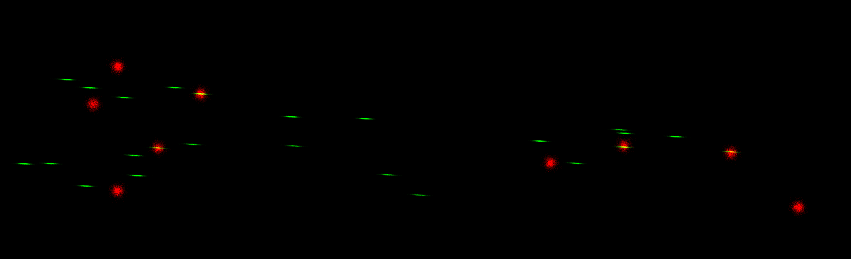
\includegraphics[width = 0.88\textwidth]{pictures/shearingBad.png}
	\caption{Affine transformation with shearing enabled. The green channel is deformed and one bead matches by chance which led to selection of this transformation.}
	\label{badshearing}
\end{figure}

\section{Accuracy of Registration}


\section{Colocalisation}
Colocalisation in wide field microscopy is a measure of the overlap of data point from different channels. It can provide information whether or not two molecules interact. With increasing resolution of the images colocalisation becomes more and more a measure of similar structures near each other. Two structures can't be at the very same position in the cell. The colorcomposer software provides both global and local colocalisation measurements.
\subsection{Global colocalisation}
The most common colocalisation measure is Pearsons correlation coefficient \cite{pearson}. It is given as:
\begin{align}
\text{Pearson correlation coefficient =}\frac{\sum ^n _{i=1}(X_i - \bar{X})(Y_i - \bar{Y})}{\sqrt{\sum ^n _{i=1}(X_i - \bar{X})^2} \sqrt{\sum ^n _{i=1}(Y_i - \bar{Y})^2}}
\end{align}
It is the ratio between the covariance between the points of two channels and their standard deviation.\newline

Also the Manders correlation coefficients $M_1$ and $M_2$ and the overlap coefficient (\cite{manders}) are calculated.
\begin{align}
M_1 =& \frac{\sum_i R_{i,\text{coloc}}}{\sum_i R_i}\\
M_2 = & \frac{sum_i G_{i,\text{coloc}}}{\sum_i G_i}
\end{align}
With $R_{i,\text{coloc}} = R_i$ if $G_i >0$ and $R_{i,\text{coloc}} = 0$ otherwise and $G_{i,\text{coloc}} = G_i$ if $R_i >0$ and $G_{i,\text{coloc}} = 0$. $G_i$, $R_i$ are the intensities of the pixel of the green and red channel.
\begin{align}
\text{overlap coefficient} = \frac{\sum_i R_i \cdot G_i}{\sqrt{\sum_i left(R_i\right)^2 \cdot \sum_i \left(G_i\right)^2}} 
\end{align}

\subsection{Local colocalisation}
\subsection{Validation of colocalisation approaches}
"Image set CBS001RGM-CBS010RGM from the Colocalization Benchmark Source
(www.colocalization-benchmark.com) was used to validate colocalization."
